\documentclass[a4paper]{article}

\usepackage[portuguese]{babel}
\usepackage[utf8]{inputenc}
\usepackage[T1]{fontenc}

\newcommand{\documentTitle}{Braitenberg Vehivles} %Macro definition
\newcommand{\documentAuthors}{João Rafael (2008111876) \and José Ribeiro (2008112181)} %Macro definition

\title{\documentTitle}
\author{\documentAuthors{}}

\usepackage{hyperref}
\hypersetup{
	pdftitle = \documentTitle
	,pdfauthor = \documentAuthors
	,pdfsubject = {Introduction to Artificial Inteligence Project \#1 Report}
	,pdfkeywords = {Artificial Inteligence Project} {Reactive Agents} {Braitenberg Vehicles}
	,pdfborder = {0 0 0}
}

\usepackage{amsmath}
\usepackage{wrapfig}
\usepackage{array}
\usepackage{anysize}
\usepackage{lscape}
\usepackage[pdftex]{graphicx}

\marginsize{3.5cm}{3.5cm}{3cm}{3cm}

\makeatletter

\begin{document}
\maketitle
\cleardoublepage

\tableofcontents
\cleardoublepage

\setlength{\parindent}{1cm}
\setlength{\parskip}{0.3cm}

\section{Introduction}
% TODO

\cleardoublepage
\section{Breve Libraries}
% TODO
Como referenciado na documentação da biblioteca Breve, o código Python fornecido é obtido através da compilação de código Steve.
Assim, esta biblioteca está pouco optimizada na medida em que não utiliza todas as potencialidades da linguagem. 
Por isso decidimos efectuar algumas alterações

\subsection{Constructors with parameters}

\subsection{Object distance}
\indent \indent Para implementar correctamente os sensores, é necessário calcular a distância entre dois objectos.
Para o cálculo desta distância as bibliotecas originais apenas teem em conta a distância euclidiana entre os centros.
No entanto esta aproximação não é suficiente quando os objectos teem dimensões elevadas.

\subsubsection{Point - Sphere}
\indent \indent Por definição todos os pontos da superficie esférica estão à mesma distância do centro.
Desta forma a solução para o caso das esferas é apenas considerar a distância entre os centros e subtrair o raio da esfera.

\subsubsection{Point - Box}
\indent \indent Uma solução eficiente para este caso consiste em utilizar o algoritmo de Arvo como \\ descrito em  \footnote[1]{\url{http://www.gamasutra.com/view/feature/3383/simple_intersection_tests_for_games.php?page=4}}.
No entanto este algoritmo necessita que a Box esteja alinhada com os eixos.
Como este não é originalmente o caso é necessário transformar as coordenadas do ponto no referencial original $O$ para o referencial da box $B$.
Esta transformação é obtida através do produto de matrizes:

\[
 	\begin{bmatrix}
		P_{x}' \\
		P_{y}' \\
		P_{z}' \\
		1 
	\end{bmatrix}
	=
	\begin{bmatrix}
		x_{x} & x_{y} & x_{z} & \vline & O_{x}	\\
		y_{x} & y_{y} & y_{z} & \vline & O_{y}	\\
		z_{x} & z_{y} & z_{z} & \vline & O_{z}	\\
		0 & 0 & 0 & \vline & 1 	\\
	\end{bmatrix}
	*
 	\begin{bmatrix}
		P_{x} \\
		P_{y} \\
		P_{z} \\
		1 
	\end{bmatrix}
\]

Onde $x, y, z$ são os versores do referencial $B$ em relação ao referencial $O$ e $O_{x}, O_{y}, O_{z}$ são as coordenadas da origem do rerefencial O nas coordenadas do referencial B. 

\cleardoublepage
\subsection{Activators}
\indent \indent O veiculos de Braitenberg como definidos na literatura apenas permitem relacionar um sensor directamente com uma roda.
Esta abordagem necessita a replicação de sensores quando se pretende que tenha influência em mais que uma roda.
Para evitar esta duplicação introduzimos o conceito de \emph{Activador}. 

%TODO

\subsection{Sensor rotation and initialization}
\indent \indent 

\subsection{Multibody collision handlers (Proxies, and Real's parents )}
\indent \indent

\cleardoublepage
\section{Sensors}

\subsection{Light}

\begin{wrapfigure}{r}{0.5\textwidth}
	\vspace{-30pt}
	\begin{center}
		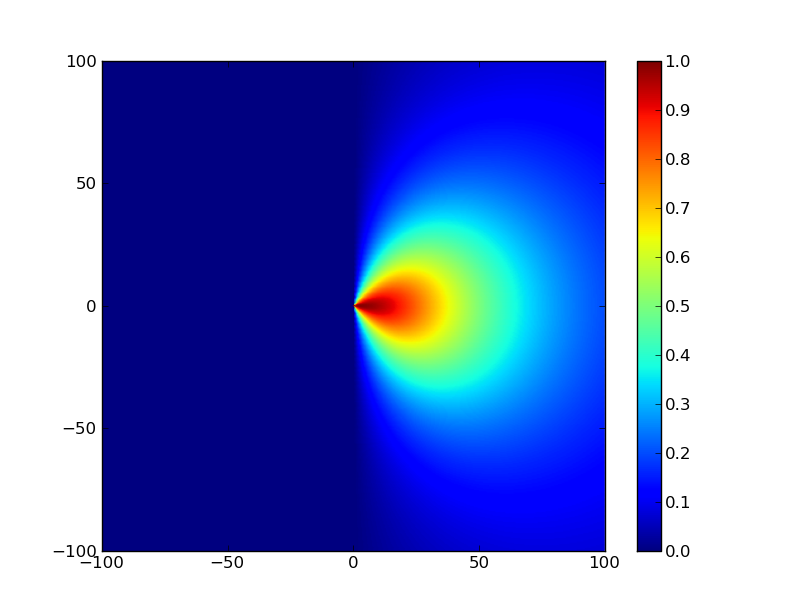
\includegraphics[width=0.48\textwidth]{graphs/light.png}
	\end{center}
	\vspace{-30pt}
	\caption{Light: $bias=50$ $\alpha=\pi/2$}
\end{wrapfigure}

\subsection{Distance}
\begin{wrapfigure}{r}{0.5\textwidth}
	\vspace{-30pt}
	\begin{center}
		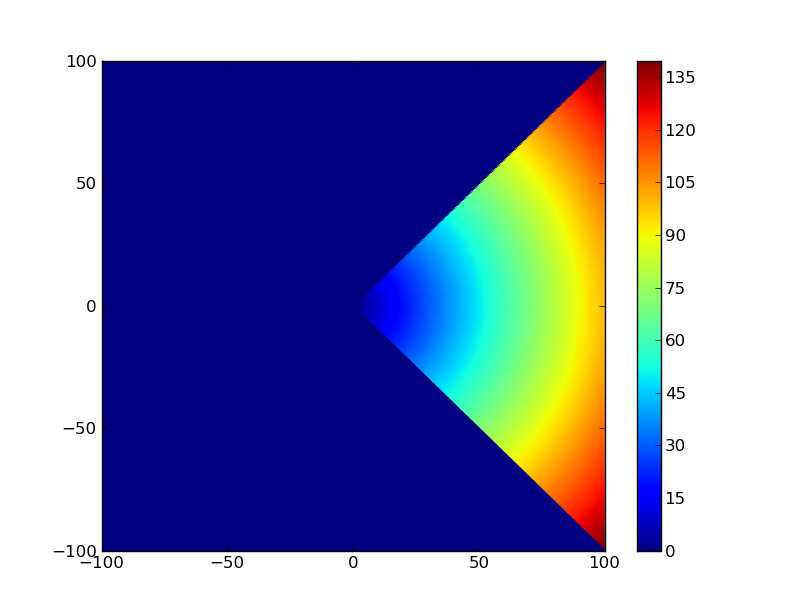
\includegraphics[width=0.48\textwidth]{graphs/distance.png}
	\end{center}
	\vspace{-30pt}
	\caption{Distance: $\alpha=\pi/4$}
\end{wrapfigure}

\subsection{Proximity}
\begin{wrapfigure}{r}{0.5\textwidth}
	\vspace{-30pt}
	\begin{center}
		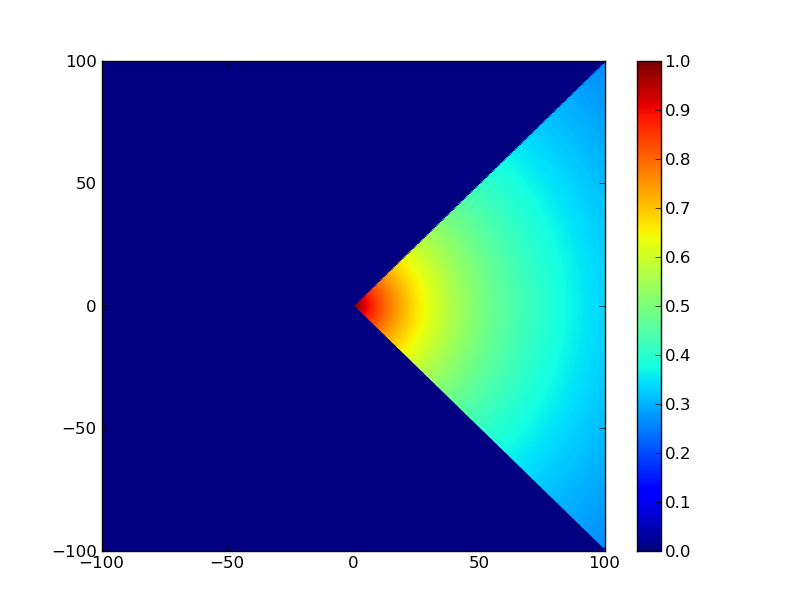
\includegraphics[width=0.48\textwidth]{graphs/proximity.png}
	\end{center}
	\vspace{-30pt}
	\caption{Proximity: $bias=50$ $\alpha=\pi/4$}
\end{wrapfigure}

\subsection{Smell}
\begin{wrapfigure}{r}{0.5\textwidth}
	\vspace{-30pt}
	\begin{center}
		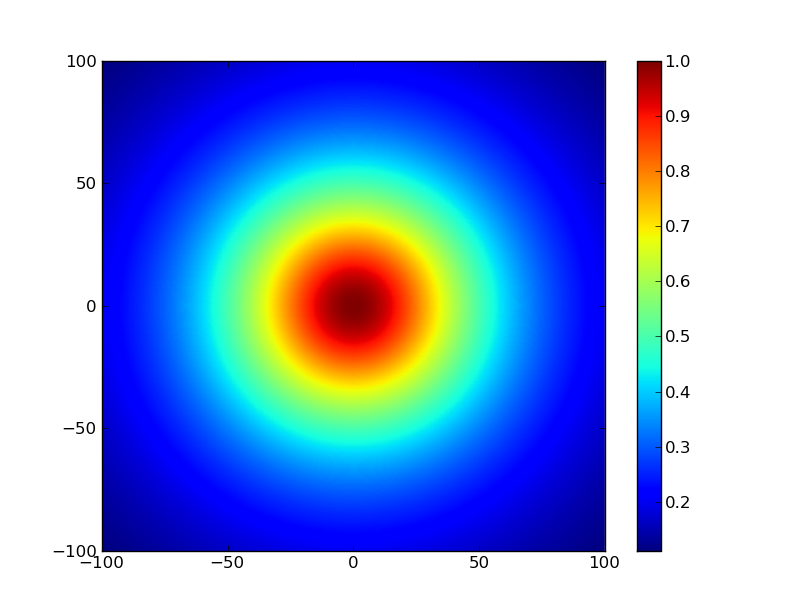
\includegraphics[width=0.48\textwidth]{graphs/smell.png}
	\end{center}
	\vspace{-30pt}
	\caption{Smell: $bias=50$}
\end{wrapfigure}

\subsection{Sound}
\begin{wrapfigure}{r}{0.5\textwidth}
	\vspace{-30pt}
	\begin{center}
		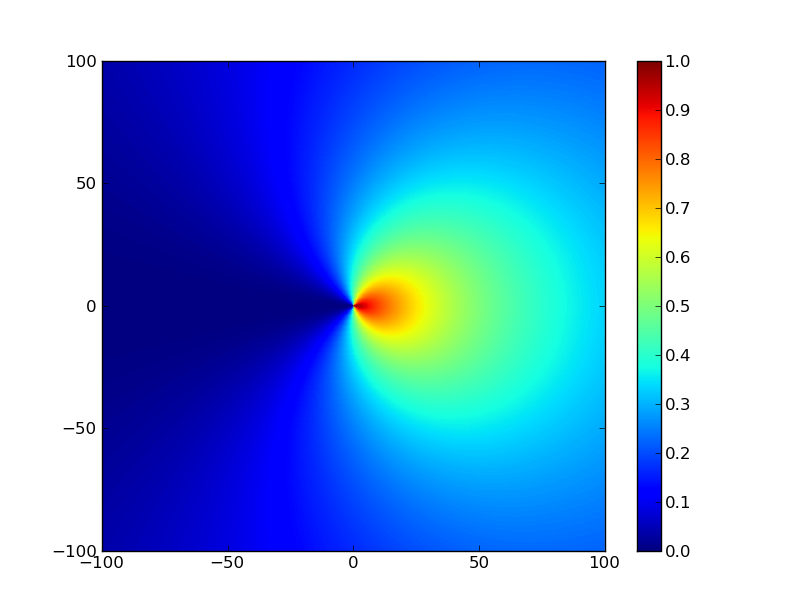
\includegraphics[width=0.48\textwidth]{graphs/cardioid.png}
	\end{center}
	\vspace{-30pt}
	\caption{Sound: $bias=50$}
\end{wrapfigure}

% TODO \subsection{Beam}

\cleardoublepage
\section{Vehicles}
\subsection{Eight}
\begin{wrapfigure}{r}{0.5\textwidth}
	\begin{center}
		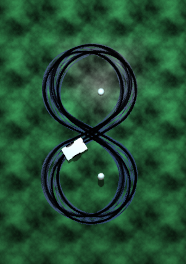
\includegraphics[width=0.48\textwidth]{trail/eight.png}
	\end{center}
	\caption{Trail of the eight vehicle}
\end{wrapfigure}

\subsection{Ellipse}
\begin{wrapfigure}{r}{0.5\textwidth}
	\begin{center}
		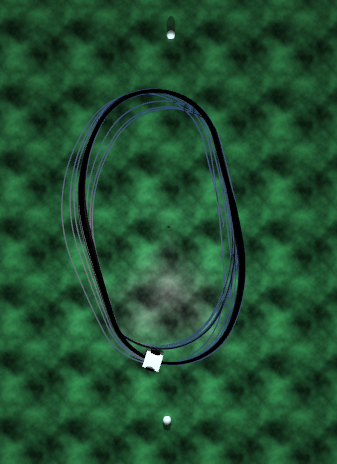
\includegraphics[width=0.48\textwidth]{trail/ellipse.png}
	\end{center}
	\caption{Trail of the ellipse vehicle}
\end{wrapfigure}

\subsection{Braitenberg 3c}

\cleardoublepage
\section{Project}


\end{document}
